\section{Neural Networks and Deep Learning}

%%%%%%%%%%%%%%%%%%%%%%%%%%%
%%%%%%%%%%%%%%%%%%%%%%%%%%%
%%%%%%%%%%%%%%%%%%%%%%%%%%%
%%%%%%%%%%%%%%%%%%%%%%%%%%%
%%%%%%%%%%%%%%%%%%%%%%%%%%%
\subsection{Introduction}

A neural network is a ML model inspired by the network of biological neurons in our brains.

NNs are versatile, powerful, and scalable.
Consequently, they frequently outperform other ML techniques on very large and complex problems.
NNs are at the very core of Deep Learning.

\textbf{Threshold Logic Units (TLUs)} are the building block of neural networks (i.e. the neurons):
\begin{itemize}
\vspace{-4.0mm}

\item
First, they perform a weighted sum of the inputs, $z = \sum w_i x_i$

\item
\vspace{-2.0mm}
Then they apply an \textit{activation function} to that sum, $h_{\boldsymbol{w}}(\boldsymbol{x}) = \phi(z)$, and output the result.\newline
\begin{figure}[ht]
\centering
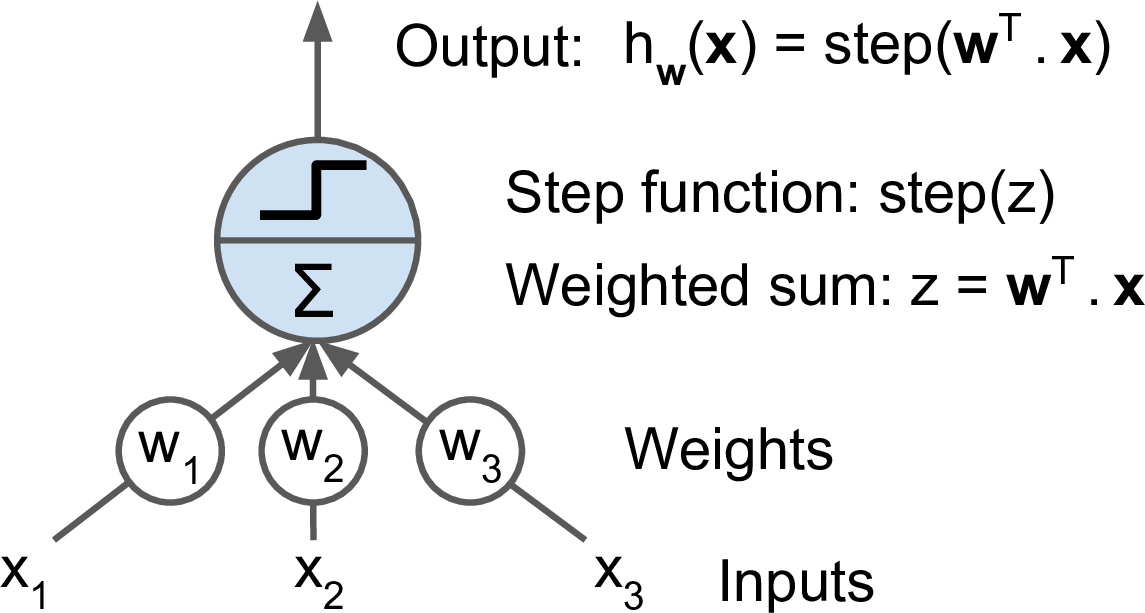
\includegraphics[width=0.50\textwidth]{./images/TLU.png}
\end{figure}

\item
\vspace{-2.0mm}
Traditionally, the activation function was a heavyside step function.
However, in order to perform Gradient Descent on a NN,
a differentiable function was needed instead.\newline
- The default has become the Rectified Linear Unit function: ReLU(z) = max(0,z)\newline
- The logistic function and hyperbolic tangent function are also popular choices.
\end{itemize}
\vspace{-2.0mm}


\textbf{Multilayer Perceptrons (MLPs)} are composed of multiple TLUs as depicted in the diagram.\newline
\textit{The bias neurons are shown, but usually they are implicit.}
\begin{figure}[ht]
\centering
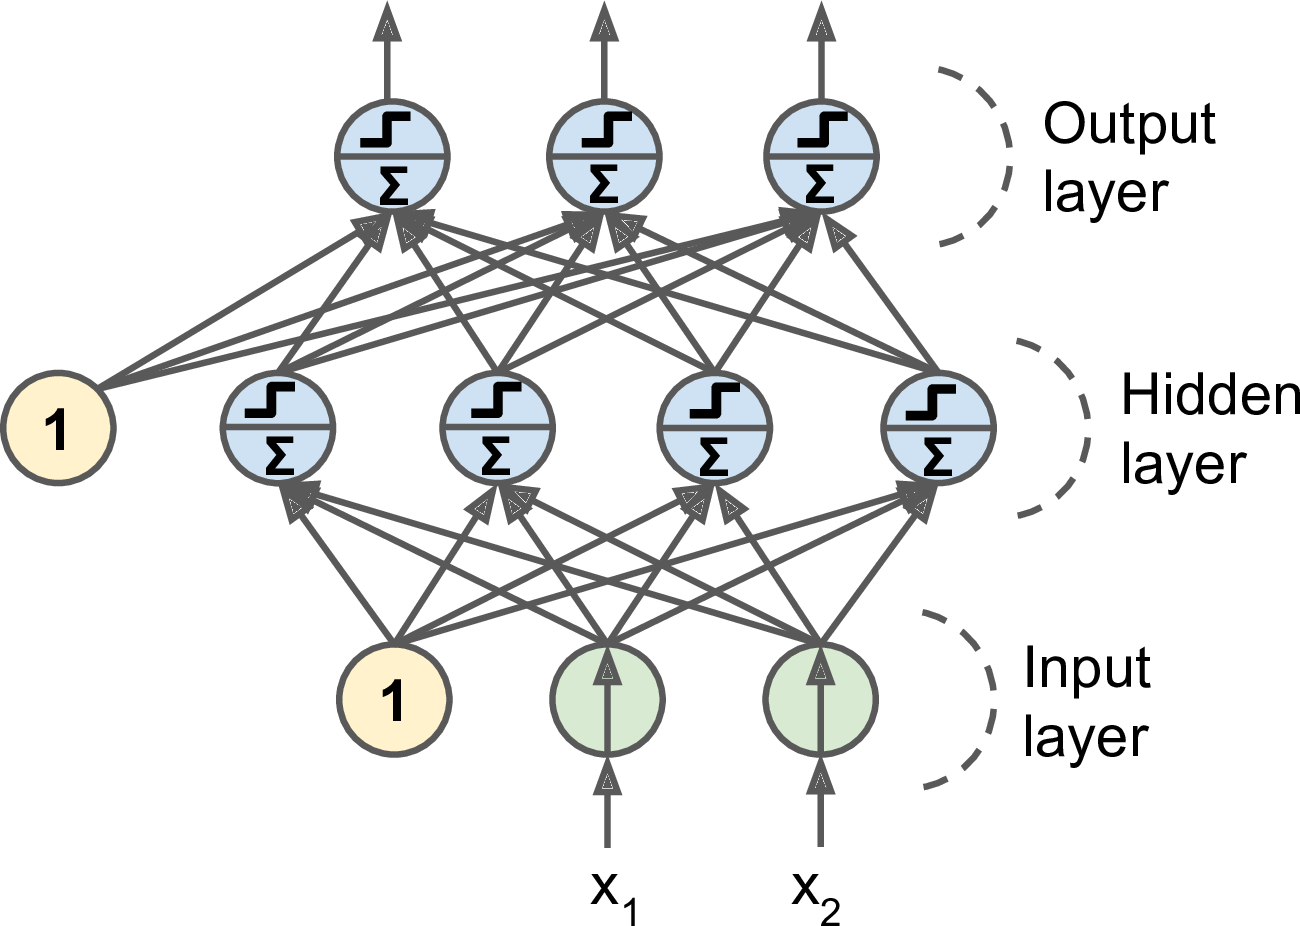
\includegraphics[width=0.50\textwidth]{./images/MLP.png}
\end{figure}

\vspace{-6.0mm}
\begin{itemize}
\item
When there's a deep stack of hidden layers, it is called a \textit{deep neural network (DNN)}.
\item
\vspace{-2.0mm}
Layers close to the input layer are called the \textit{lower layers}\newline
Layers close to the output layer are called the \textit{upper layers}.
\item
\vspace{-2.0mm}
When all the neurons in a layer are connected to every neuron in the previous layer,\newline
the layer is called a \textit{fully connected layer} or a \textit{dense layer}.
\item
\vspace{-2.0mm}
The signal flows only in one direction $=$ \textit{feedforward neural network (FNN)}.
\item
\vspace{-2.0mm}
Without the activation functions, all you would get is a linear model!
\end{itemize}

\newpage
\textbf{Training NNs: Backpropagation}.\newline
In just two passes through the network (one forward, one backward)
the backpropagation algorithm is able to compute the gradient of the network's error
with regard to every single model parameter (i.e. the connection weights),
allowing Gradient Descent to be used to train the NN.

\vspace{-5.0mm}
\begin{itemize}
\item
It handles one mini-batch at a time. The bigger the batch size, the more memory required.

\item
\vspace{-2.0mm}
\textit{The forward pass}.
Each mini-batch is passed through the network.
The output of every neuron is computed and preserved (for every instance in the mini-batch).

\item
\vspace{-2.0mm}
The network's output error is measured.

\item
\vspace{-2.0mm}
\textit{The reverse pass}.
The error gradient across all the connection weights is measured
by propagating the error gradient backward through the network.

\item
\vspace{-2.0mm}
An \textbf{iteration} = one forward-backward pass using one mini-batch.\newline
An \textbf{epoch} = one forward-backward pass of \textit{all} the training set examples.\newline
If you have 2000 training examples, and your batch size is 500...\newline
$\rightarrow$ then it will take 4 iterations to complete 1 epoch.

\item
\vspace{-2.0mm}
It is important to randomly initialize all the hidden layer's connection weights.\newline
This breaks the symmetry and allows backpropagation to train a diverse team of neurons.

\end{itemize}

\textbf{Regression MLPs: Summary}

\begin{tabular}{ |l|l| } 
\hline
Hyperparameter & Typical value \\ 
\hline
Number of input neurons & One per input feature \\ 
Number of hidden layers & Depends on the problem, but typically 1 to 5\\ 
Number of neurons per hidden layer & Depends on the problem, but typically 10 to 100\\ 
Hidden layer activation function & ReLU or SELU\\
Number of output neurons & 1 per prediction dimension\\
Output activation function & In general None (can output any range of values)\\
 & ReLU/softplus (for a positive output contraint)\\
 & Logistic/tanh (for a bounded output contraint)\\
Loss function & Typically MSE (mean squared error)\\
 & Maybe MAE (mean absolute error) when there's lots of outliers\\
\hline
\end{tabular}

\textbf{Classification MLPs: Summary}

\begin{tabular}{ |l|l| } 
\hline
Hyperparameter & Typical value \\ 
\hline
Number of input neurons & One per input feature \\ 
Number of hidden layers & Depends on the problem, but typically 1 to 5\\ 
Number of neurons per hidden layer & Depends on the problem, but typically 10 to 100\\ 
Hidden layer activation function & ReLU or SELU\\
Number of output neurons & 1 (for binary classification)\\
 & 1 per class (for multiclass classification)\\
Output activation function & Logistic (for binary classification)\\
 & Softmax (for multiclass classification)\\
Loss function & Cross entropy\\
\hline
\end{tabular}

\newpage
The architecture of an MLP for multiclass classification:

\begin{figure}[ht]
\centering
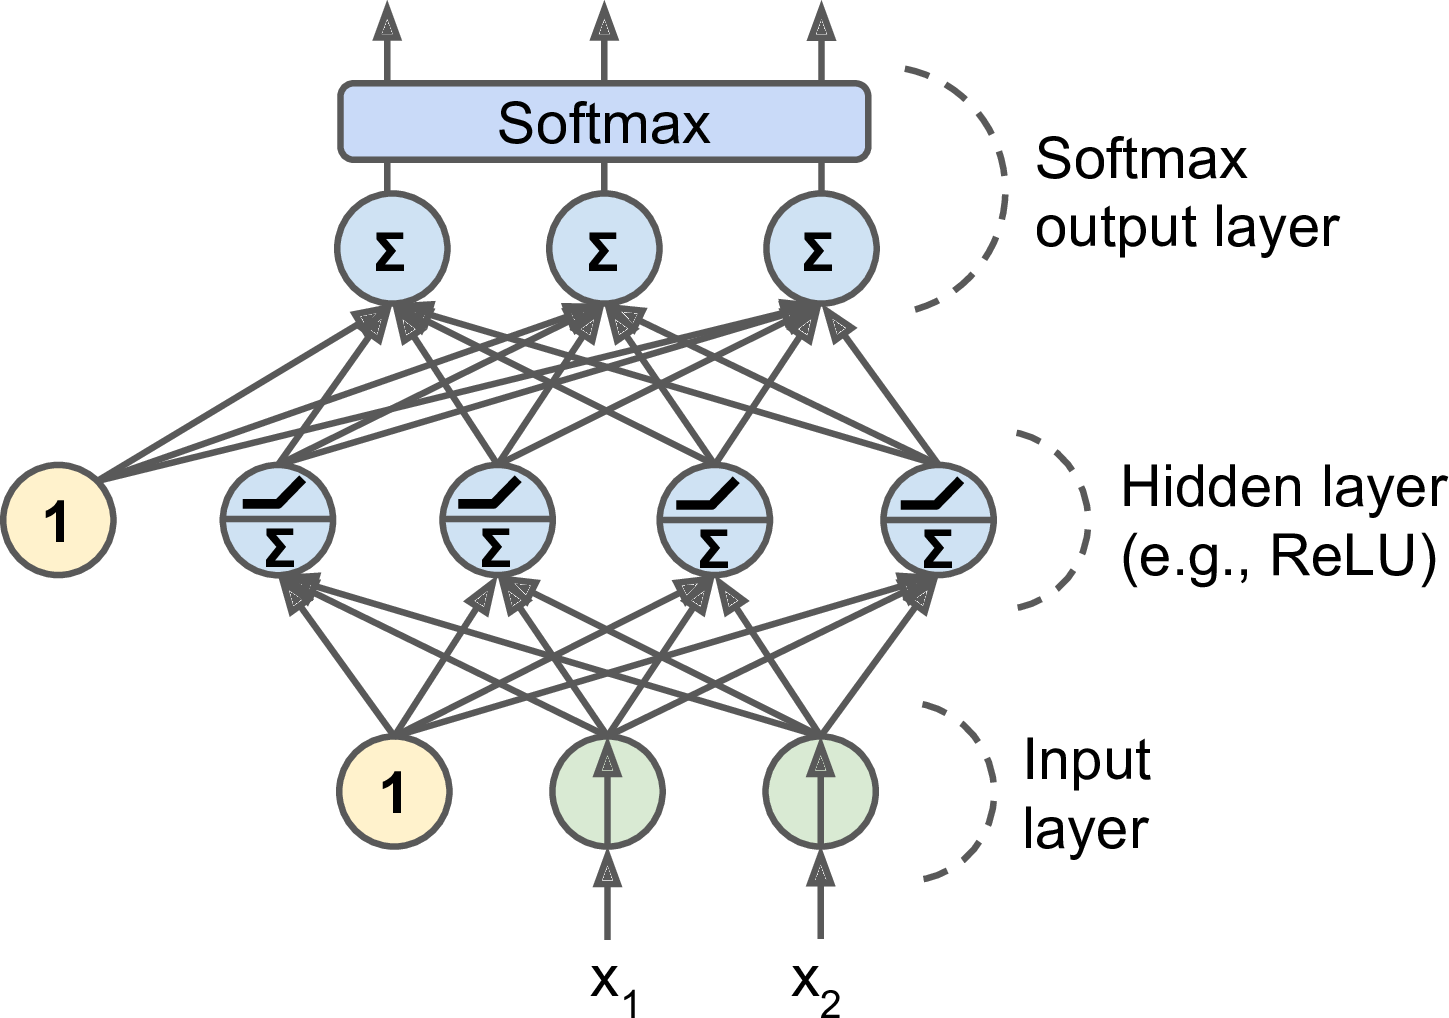
\includegraphics[width=0.50\textwidth]{./images/MLP_classification.png}
\end{figure}

%%%%%%%%%%%%%%%%%%%%%%%%%%%
%%%%%%%%%%%%%%%%%%%%%%%%%%%
%%%%%%%%%%%%%%%%%%%%%%%%%%%
%%%%%%%%%%%%%%%%%%%%%%%%%%%
%%%%%%%%%%%%%%%%%%%%%%%%%%%

\subsection{Implementing MLPs with Keras}

The following code creates a classification MLP with:
\vspace{-5.0mm}
\begin{itemize}
\item
An input layer with 784 neurons, where each instance is a $28*28$ array.
\vspace{-3.0mm}
\item
Two hidden layers (with 300 and 100 neurons, respectively).\newline
Both layers use the ReLU activation function.\newline
All the layers are connected sequentially.
\vspace{-3.0mm}
\item
10 exclusive classification outputs.
\end{itemize}

\vspace{-2.0mm}
\texttt{from tensorflow import keras}\newline
\texttt{model = keras.models.Sequential()}\newline
\texttt{model.add(keras.layers.Flatten(input\char`_shape=[28,28]))}\newline
\texttt{model.add(keras.layers.Dense(300, activation=\textquotesingle relu\textquotesingle))}\newline
\texttt{model.add(keras.layers.Dense(100, activation=\textquotesingle relu\textquotesingle))}\newline
\texttt{model.add(keras.layers.Dense(10, activation=\textquotesingle softmax\textquotesingle))}\newline
\vspace{-2.0mm}

For binary classification, use \texttt{activation=\textquotesingle sigmoid\textquotesingle} (i.e. the logistic function)\newline
For regression, the output layer would be:~\texttt{model.add(keras.layers.Dense(1))}

The following will give a summary of your model:\newline
\textit{Note that `None' in the Output Shape means that the batch size can be anything.}\newline
\texttt{model.summary()}

Each model layer is its own object:\newline
\texttt{input = model.layers[0]}\newline
\texttt{hidden\char`_1 = model.layers[1]}\newline
\texttt{hidden\char`_2 = model.layers[2]}\newline
\texttt{output = model.layers[3]}

Each layer manages its own connection weights between the layers neurons and their inputs:\newline
\texttt{weights, biases = hidden\char`_2.get\char`_weights()}

Notice that the connection weights are randomly initialized (this is required to break symmetry)
and the biases are initialized to zero.\newline
\textit{Sometimes you may want to use a different initialization method (information provided later).}

\newpage
\textbf{Compilation}\newline
After a model is created, you must specify the loss function and the optimizer to use:\newline
\texttt{model.compile(loss=\textquotesingle sparse\char`_categorical\char`_crossentropy\textquotesingle,}\newline
\texttt{.~~~~~~~~~~~~~optimizer=\textquotesingle sgd\textquotesingle,}\newline
\texttt{.~~~~~~~~~~~~~metrics=[\textquotesingle accuracy\textquotesingle]) \# these are optional}

For binary classification: \texttt{loss=\textquotesingle binary\char`_crossentropy\textquotesingle}\newline
For regression: \texttt{loss=\textquotesingle mean\char`_squared\char`_error\textquotesingle}

Note that the optimizer is equivalent to: \texttt{optimizer=keras.optimizers.SGD(lr=0.01)}\newline
\textit{Sometimes you may want to use more efficient optimizers (information provided later).}\newline

\textbf{Training}\newline
\texttt{history = model.fit(X, y, epochs=30, validation\char`_split=0.1)}

- The \texttt{fit()} method returns a History object containing meta-data about the training.\newline
- If not stated, the \texttt{epochs} parameter will default to one (not enough for convergence).\newline
- If not stated, the \texttt{validation\char`_split} parameter will be zero (i.e no cross validation).

Use the History object to plot the learning curves:\newline
\texttt{import pandas as pd}\newline
\texttt{import matplotlib.pyplot as plt}\newline
\texttt{pd.DataFrame(history.history).plot(figsize=(12,8))}\newline
\texttt{plt.grid(True)}\newline
\texttt{plt.gca().set\char`_ylim(0,1)}\newline
\texttt{plt.show()}\newline
\textit{Note that the validation error is computed at the \underline{end} of each epoch,
whilst the training error is computed using a running mean \underline{during} each epoch.}

To continue training, just call the \texttt{fit()} method again. Note the following:\newline
- This will create a new History object (rather than appending).\newline
- You can update the model compilation parameters before the additional training.\newline

\textbf{Evaluation}\newline
Estimate the generalization error using the test set:\newline
\texttt{model.evaluate(X\char`_test, y\char`_test)}

Make predictions as follows:\newline
\texttt{y\char`_proba = model.predict(X\char`_new)}\newline
\texttt{y\char`_pred ~= np.argmax(model.predict(X\char`_new), axis=-1)}\newline

\textbf{Saving and Loading}\newline
The following saves a model's architecture, parameters, and optimizer:\newline
\texttt{model.save(\textquotesingle my\char`_keras\char`_model.h5\textquotesingle)}

The following loads a model:\newline
\texttt{model = keras.models.load\char`_models(\textquotesingle my\char`_keras\char`_model.h5\textquotesingle)}

You can also save your model at regular checkpoints during training...

\newpage
\textbf{Callbacks}\newline
The \texttt{fit()} method accepts a \textit{callbacks} argument
(a list of objects called \underline{during} training).

The following saves your model at regular intervals (default = end of each epoch):\newline
\texttt{save\char`_cb = keras.callbacks.ModelCheckpoint(\textquotesingle my\char`_keras\char`_model.h5\textquotesingle)}\newline
\texttt{history = model.fit(X, y, epochs=10, callbacks=[save\char`_cb])}

Moreover, if you use a validation set during training,
you can ensure your model only saves when the performance on the validation set is the best so far (i.e implicit early stopping):
\texttt{save\char`_cb = keras.callbacks.ModelCheckpoint(\textquotesingle my\char`_keras\char`_model.h5\textquotesingle,\newline
.~~~~~~~~~~~~~~~~~~~~~~~~~~~~~~~~~~~~~~~~~save\char`_best\char`_only=True)}\newline
\texttt{history = model.fit(X, y, epochs=100, validation\char`_split=0.1,\newline
.~~~~~~~~~~~~~~~~~~~callbacks=[save\char`_cb])}

Explicit early stopping can be implemented with the following callback:\newline
\texttt{early\char`_stop\char`_cb = \newline keras.callbacks.EarlyStopping(patience=10, restore\char`_best\char`_weights=True)}

%%%%%%%%%%%%%%%%%%%%%%%%%%%
%%%%%%%%%%%%%%%%%%%%%%%%%%%
%%%%%%%%%%%%%%%%%%%%%%%%%%%
%%%%%%%%%%%%%%%%%%%%%%%%%%%
%%%%%%%%%%%%%%%%%%%%%%%%%%%
\subsection{Fine-Tuning Neural Network Hyperparameters}

The flexibility of NNs is also one of their drawbacks,
there are many hyperparameters to tune:

\vspace{-5.0mm}
\begin{itemize}
\item
\textbf{Learning rate:} very low = $10^{-5}$, keras default = 0.01, very high = 10.\newline
\textit{Always retune this after changing another hyperparameter.}
\item
\textbf{Optimizer:} there are better options out there than mini-batch gradient descent...
\item
\textbf{Batch size:} keras default = 32 (large batch sizes can lead to training instabilities).
\item
\textbf{Hidden layer activation function:} ReLU is a good default in general.
\item
\textbf{Number of hidden layers:} for most problems, you can start with just one or two.
\item
\textbf{Number of neurons:} in general, use the same number for all hidden layers.\newline
\textit{It can sometimes help to make the first hidden layer bigger than the others.}
\item
\textbf{Keras Tuner:} use this library to tune hyperparameters \textit{(keras-team.github.io/keras-tuner/)}
\item
\textbf{Tip:} it's often simpler to pick a model with more layers and neurons than you actually need,
then use early stopping \& other regularization techniques to prevent overfitting.
\end{itemize}
% 
\textbf{Number of hidden layers}\newline
If it has enough neurons, one hidden layer can theoretically model the most complex functions.
% 
However, for complex problems,
deep networks have a much higher \textit{parameter efficiency} than shallow ones:
they can model complex functions using exponentially fewer neurons,
allowing them to reach much better performance with the same amount of training data.
% 
This is because real-world data is often structured in a hierarchial way,
and deep neural networks take advantage of this:\newline
- Lower hidden layers model low-level structures (e.g. line segments).\newline
- Intermediate hidden layers combine these to model intermediate-level structures (e.g. shapes).\newline
- The highest hidden layers combine these to model high-level structures (e.g. faces).\newline
- \textit{Transfer learning} is where you `borrow' the lower layers from a previously trained model.

%%%%%%%%%%%%%%%%%%%%%%%%%%%
%%%%%%%%%%%%%%%%%%%%%%%%%%%
%%%%%%%%%%%%%%%%%%%%%%%%%%%
%%%%%%%%%%%%%%%%%%%%%%%%%%%
%%%%%%%%%%%%%%%%%%%%%%%%%%%
\subsection{Training Deep Neural Networks}

What if you need to tackle a complex problem,
such as detecting hundreds of types of objects in high-resolution images?
% 
You may need to train a much deeper DNN,
perhaps with 10+ layers,
each containing hundreds of neurons.
% 
You might then experience the following problems:

\vspace{-5.0mm}
\begin{itemize}
\item
The \textit{vanishing gradients} or \textit{exploding gradients} problem.
This is when gradients grow ever smaller (or ever larger)
when flowing backward through the DNN during training.
This makes it very hard to train the lower layers.
\vspace{-2.0mm}
\item
Training may be extremely slow.
\vspace{-2.0mm}
\item
A model with millions of parameters risks severly overfitting the training set,
especially if there are not enough training instances or if they are too noisy.
\end{itemize}

\textbf{\underline{The Vanishing Gradients Problem}}\newline
% 
Gradients often get ever smaller as the backpropagation progresses down to the lower layers.
Consequently, the update leaves the lower layers' connection weights virtually unchanged.\newline
This means the training never converges on a good solution.

For the signal to flow properly,
we need the outputs (forward pass) and the gradient (reverse pass) of all the layers to have equal variance.\newline

\textbf{*** Weight Initialization ***}\newline
$fan_{\textrm{in}}$ = the number of inputs into a layer.\newline
$fan_{\textrm{out}}$ = the number of neurons in a layer.\newline
$fan_{\textrm{avg}} = (fan_{\textrm{in}} + fan_{\textrm{out}})/2$.

The connection weights of each layer should be initialized randomly by one of the following:\newline
- Normal distribution with mean 0 and variance $\sigma^2$\newline
- Uniform distribution between $-r$ and $+r$, where $r=\sqrt{3 \sigma^2}$ 

\begin{tabular}{ l|l|l } 

Initialization & Layer Activation function & $\sigma^2$ \\ 
\hline
Glorot & None, tanh, logistic, softmax & $1/fan_{\textrm{avg}}$\\
He & ReLU and variants & $2/fan_{\textrm{in}}$\\
LeCun & SELU & $1/fan_{\textrm{in}}$\\
\end{tabular}

By default, Keras uses Glorit initialization with a uniform distribution when you create a layer.\newline
You can override this like so:\newline
\texttt{keras.layers.Dense(10, activation=\textquotesingle relu\textquotesingle, kernel\char`_initializer=\textquotesingle he\char`_normal\textquotesingle)}
\texttt{keras.layers.Dense(30, activation=\textquotesingle relu\textquotesingle, kernel\char`_initializer=\textquotesingle he\char`_uniform\textquotesingle)}\newline

\textbf{*** Activation Functions ***} \textit{they get better as you go down...}

\textbf{Logistic:} saturates at 0 or 1, with a derivative extremely close to 0. Function has a mean of 0.5.\newline
\textbf{Tanh:} saturates at -1 or 1, with a derivative extremely close to 0. Function has a mean of 0.

\textbf{ReLU:} does not saturate for positive values, and is fast to compute.\newline
During training, some neurons can effectively die (they stop outputting anything other than 0).\newline
This happens when the weighted sum of its inputs are negative for all instances in the training set.
The weights are then no longer updated by Gradient Descent as the gradient is always zero.

\textbf{LeakyReLU} = $\textrm{max}(\alpha z, z)$.
The hyperparameter $\alpha$, typically set to 0.01, defines how much the function `leaks' for $z<0$.
This small slope ensures that leaky ReLUs never die.

\textbf{Exponential Linear Unit (ELU)} = $\alpha(e^z - 1)$ if $z < 0$.
The hyperparameter $\alpha$, typically set to unity, defines the output as $z \rightarrow -\infty$.
This function has a mean value closer to zero and is differentiable at $z=0$.
The use of the exponential function makes it slower to compute.

\textbf{Scaled ELU (SELU):} a scaled variant of ELU ($\alpha = 1.67$ and $scale = 1.05$).\newline
If you build a DNN composed of a sequential stack of dense layers,
and if all hidden layers use the SELU activation function,
then the network will \textit{self-normalize}:
the output of each layer will preserve a mean of 0 and a standard deviation of 1 during training. Conditions:\newline
- The input features must be standardized.\newline
- Every hidden layer's weights must be initialized with LeCun normal initialization. E.g.\newline
\texttt{layers.Dense(10, activation=\textquotesingle selu\textquotesingle, kernel\char`_initializer=\textquotesingle lecun\char`_normal\textquotesingle)}\newline

\textbf{*** Batch Normalization ***}

Although your weight initialization and activation function choice can significantly reduce the danger of vanishing/exploding gradients at the beginning of training,
it doesn't guarantee that they won't come back as the training progresses... Batch Normalization (BN) addresses this.

BN adds an operation in the model just before/after the activation function of each hidden layer.
For each neuron, this operation zero-centres and normalizes the mini-batch instance values.\newline
The results are scaled and shifted using two parameter vectors (two parameters per neuron).\newline
The scaling parameter, $\boldsymbol{\gamma}$, and the shifting parameter, $\boldsymbol{\beta}$, are learnt during training.

\underline{Notes:}\newline
- BN acts like a regularizer, reducing the need for other regularization techniques.\newline
- After training, when making a prediction on a single instance,
an estimated value of the mean and standard deviation for each neuron is used.

\texttt{...}\newline
\texttt{model.add(keras.layers.Flatten(input\char`_shape=[28,28]))}\newline
\texttt{model.add(keras.layers.BatchNormalization())}\newline
\texttt{model.add(keras.layers.Dense(300, activation=\textquotesingle relu\textquotesingle))}\newline
\texttt{model.add(keras.layers.BatchNormalization())}\newline
\texttt{...}\newline

\textbf{*** Gradient Clipping ***}

This technique ensures gradients never exceed some threshold during backpropagation.\newline
It's typically used to mitigate exploding gradients in RNNs.

Each individual gradient component is clipped between -1.0 and 1.0:\newline
\texttt{optimizer = keras.optimizers.SGD(clipvalue=1.0)}

Clip the magnitude of the gradient to 1.0:\newline
\texttt{optimizer = keras.optimizers.SGD(clipnorm=1.0)}

\newpage

\textbf{*** Reusing Pretrained Layers ***}

It is generally not a good idea to train a very large DNN from scratch.
Instead, you should always try to find an existing neural network that accomplishes a similar task,
then reuse the lower layers. This is called \textit{transfer learning}.
It speeds up training and requires less data.\newline

\textbf{\underline{Faster Optimizers}}

Huge training speed boosts can be achieved using a faster optimizer than Gradient Descent:

\textbf{Momentum Optimization:}\newline
$\boldsymbol{m} \leftarrow \beta \boldsymbol{m} - \eta \nabla_{\boldsymbol{\theta}} J (\boldsymbol{\theta})$\newline
$\boldsymbol{\theta} \leftarrow \boldsymbol{\theta} + \boldsymbol{m}$\newline
\texttt{optimizer = keras.optimizers.SGD(lr=0.001, momentum=0.9)}\newline

\textbf{Nesterov Accelerated Gradient (NAG):}\newline
$\boldsymbol{m} \leftarrow \beta \boldsymbol{m} - \eta \nabla_{\boldsymbol{\theta}} J (\boldsymbol{\theta} + \beta \boldsymbol{m})$\newline
$\boldsymbol{\theta} \leftarrow \boldsymbol{\theta} + \boldsymbol{m}$\newline
\texttt{optimizer = keras.optimizers.SGD(lr=0.001, momentum=0.9, nesterov=True)}\newline
Generally, this is faster than regular momentum optimization.\newline

\textbf{RMSProp:}\newline
$\boldsymbol{s} \leftarrow \beta \boldsymbol{s} - (1 - \beta) \nabla_{\boldsymbol{\theta}} J (\boldsymbol{\theta}) \otimes \nabla_{\boldsymbol{\theta}} J (\boldsymbol{\theta})$\newline
$\boldsymbol{\theta} \leftarrow \boldsymbol{\theta} - \eta  \nabla_{\boldsymbol{\theta}} J (\boldsymbol{\theta}) \oslash \sqrt{\boldsymbol{s} + \epsilon} $\newline
\texttt{optimizer = keras.optimizers.RMSprop(lr=0.001, rho=0.9)}\newline
Converges quicker than NAG, but convergence quality might be worse.\newline

\textbf{Adaptive Moment Estimation (Adam):}\newline
$\boldsymbol{m} \leftarrow \beta_1 \boldsymbol{m} - (1 - \beta_1) \nabla_{\boldsymbol{\theta}} J (\boldsymbol{\theta})$\newline
$\boldsymbol{s} \leftarrow \beta_2 \boldsymbol{s} - (1 - \beta_2) \nabla_{\boldsymbol{\theta}} J (\boldsymbol{\theta}) \otimes \nabla_{\boldsymbol{\theta}} J (\boldsymbol{\theta})$\newline
$\widehat{\boldsymbol{m}} \leftarrow \frac{\boldsymbol{m}}{1-\beta_1}$\newline
$\widehat{\boldsymbol{s}} \leftarrow \frac{\boldsymbol{m}}{1-\beta_2}$\newline
$\boldsymbol{\theta} \leftarrow \boldsymbol{\theta} + \eta \, \widehat{\boldsymbol{m}} \oslash \sqrt{\widehat{\boldsymbol{s}} + \epsilon}$\newline
\texttt{optimizer = keras.optimizers.Adam(lr=0.001, beta\char`_1=0.9, beta\char`_2=0.999)}\newline
Often preferred to RMSProp.

Note that since RMSProp and Adam have an adaptive learning rate,
less tuning of the learning rate hyperparameter is required (you can often just use the default $\eta=0.001$).\newline

\textbf{*** Learning Rate Scheduling ***}\newline
If you start with a large learning rate and then reduce it once training stops making fast progress,
you can reach a good solution faster than with the optimal constant learning rate.

\textit{Power scheduling:} $\eta(t) = \eta_0 \, / \, (1 + t/s)$ where $t$ is the iteration number.\newline
\texttt{keras.optimizers.SGD(lr=0.01, decay=1e-4)} where \texttt{decay} is the inverse of $s$.\newline

\newpage

\textbf{\underline{Avoid Overfitting Through Regularization}}

We have already seen \textit{early stopping} and \textit{batch normalization} as forms of regularization.\newline

\underline{$l_1$ and $l_2$ regularization}\newline
This applies an $l_2$ regularization (factor=0.01) to a layer's connection weights.\newline
Note that you should typically to apply the same regularizer to all layers in your NN.\newline
\texttt{keras.layers.Dense(300, activation=\textquotesingle relu\textquotesingle,\newline
.~~~~~~~~~~~~~~~~~~kernel\char`_regularizer=keras.regularizers.l2(0.01)))}\newline

\underline{Dropout}\newline
At every training step, every neuron (including the input neurons, but excluding the outputs)
has a probability $p$ of being ignored.
The hyperparameter $p$ is called the \textit{dropout rate},
and is typically set between 10\% and 50\%.
After training, the neurons don't get dropped anymore (and each input connection weight is multiplied by $1-p$ to align the signal size with training).

Neurons trained with dropout:\newline
- Cannot co-adapt with their neighboring neurons.\newline
- Cannot rely excessively on just a few input neurons.\newline
- Are less sensitive to slight changes in their inputs.

This results in a more robust network that generalizes better.\newline
\textit{You can think of the final NN as an averaged ensemble of lots of smaller NNs.}

\texttt{...}\newline
\texttt{model.add(keras.layers.Flatten(input\char`_shape=[28,28]))}\newline
\texttt{model.add(keras.layers.Dropout(rate=0.2))}\newline
\texttt{model.add(keras.layers.Dense(300, activation=\textquotesingle relu\textquotesingle))}\newline
\texttt{model.add(keras.layers.Dropout(rate=0.2))}\newline
\texttt{...}\newline

Notes:\newline
- In practice, you only need to apply dropout to the top 1-3 layers (excluding the output layer).\newline
- Dropout means the loss evaluation during training can be misleading.\newline
- You need to use \textit{alpha dropout} if you are using the SELU activation function.

\newpage
%%%%%%%%%%%%%%%%%%%%%%%%%%%
%%%%%%%%%%%%%%%%%%%%%%%%%%%
%%%%%%%%%%%%%%%%%%%%%%%%%%%
%%%%%%%%%%%%%%%%%%%%%%%%%%%
%%%%%%%%%%%%%%%%%%%%%%%%%%%
\subsection{TensorFlow}

Around 95\% of use cases do not require anything other than \texttt{tf.keras} and \texttt{tf.data}.\newline
These are TensorFlow's high-level APIs.
But you might need to use the low-level API...\newline

\textbf{\underline{TensorFlow Objects and Operations}}

TensorFlow revolves around \textit{tensors}, which \textit{flow} from operation to operation.\newline
Creating tensors, and using them, is very similar to NumPy:

\texttt{import tensorflow as tf}\newline
\texttt{t = tf.constant([[1., 2., 3.], [4., 5., 6.]])} -- create a tensor.\newline
\texttt{t = tf.constant(a, dtype=tf.float32)} -- create a tensor from a NumPy array.

\texttt{t[:, 1:]} -- an example of indexing.

\texttt{t + 10} -- all sorts of tensor operations are available...\newline
\texttt{tf.square(t)}\newline
\texttt{tf.reduce\char`_mean(t)}\newline
\texttt{t @ tf.transpose(t)}

\texttt{t.dtype} -- note that TensforFlow uses 32-bit floats by default (NumPy uses 64-bit precision).\newline
Also note that TensorFlow does not perform any type conversions automatically.

TensorFlow supports several other data structures:\newline
Variables, sparse tensors, tensor arrays, ragged tensors, string tensors, sets, queues...\newline

\textbf{\underline{Computing Gradients Using Autodiff}}

Use autodiff to efficiently compute gradients. E.g this simple toy function at \texttt{(w1,w2)=(5,3)}.\newline
\texttt{def f(w1, w2):}\newline
\texttt{.~~~return 3*w1**2 + 2*w1*w2}\newline
\texttt{}\newline
\texttt{w1, w2 = tf.Variable(5.), tf.Variable(3.)}\newline
\texttt{with tf.GradientTape() as tape:}\newline
\texttt{.~~~z = f(w1, w2)}\newline
\texttt{gradients = tape.gradient(z, [w1, w2])}

The GradientTape records every operation that involves a Variable data structure.\newline
To save memory, only put the strict minimum inside the tape block.\newline
The tape is automatically erased immediately after you call its \texttt{gradient()} method.\newline

\textbf{\underline{Customizing Keras Models}}

Using TensorFlow's low-level API you can build custom:
% 
\vspace{-5.0mm}
\begin{itemize}
\item
Loss functions.
\vspace{-3.0mm}
\item
Activation functions.
\vspace{-3.0mm}
\item
Initializers.
\vspace{-3.0mm}
\item
Regularizers.
\vspace{-3.0mm}
\item
Layers and Models.
\end{itemize}

\newpage
For better performance,
you should only use vectorized TensorFlow operations.\newline

\textbf{\underline{Custom Loss Functions}}

\texttt{def my\char`_huber(y\char`_true, y\char`_pred):\newline
.~~~error = y\char`_true - y\char`_pred\newline
.~~~is\char`_small\char`_error = tf.abs(error) < 1\newline
.~~~squared\char`_loss = tf.square(error) / 2\newline
.~~~linear\char`_loss = tf.abs(error) - 0.5\newline
.~~~return tf.where(is\char`_small\char`_error, squared\char`_loss, linear\char`_loss)\newline
...\newline
model.compile(loss=my\char`_huber, optimizer=\textquotesingle adam\textquotesingle)\newline
...\newline
model.save(\textquotesingle my\char`_custom\char`_model.h5\textquotesingle)\newline
model = keras.models.load\char`_model(\textquotesingle my\char`_custom\char`_model.h5\textquotesingle,\newline
.~~~~~~~~~~~~~~~~~~~~~~~~~~~~~~~custom\char`_objects=\{\textquotesingle my\char`_huber\textquotesingle:my\char`_huber\})}\newline

If your custom loss function requires an argument,
you need to create a subclass of \texttt{keras.losses.Loss}
The \texttt{get\char`_config()} method allows the function argument value to be saved.


\texttt{class MyHuberLoss(keras.losses.Loss):\newline
.~~~def \char`_\char`_init\char`_\char`_(self, threshold=1.0, **kwargs):\newline
.~~~~~~~self.threshold = threshold\newline
.~~~~~~~super().\char`_\char`_init\char`_\char`_(**kwargs)\newline
.~~~def call(self, y\char`_true, y\char`_pred):\newline
.~~~~~~~error = y\char`_true - y\char`_pred\newline
.~~~~~~~is\char`_small\char`_error = tf.abs(error) < self.threshold\newline
.~~~~~~~squared\char`_loss = tf.square(error)/2\newline
.~~~~~~~lin\char`_loss  = self.threshold*tf.abs(error) - self.threshold**2/2\newline
.~~~~~~~return tf.where(is\char`_small\char`_error, squared\char`_loss, lin\char`_loss)\newline
.~~~def get\char`_config(self):\newline
.~~~~~~~base\char`_config = super().get\char`_config()\newline
.~~~~~~~return \{**base\char`_config, \textquotesingle threshold\textquotesingle:self.threshold\}\newline
...\newline
model.compile(loss=MyHuberLoss(2.), optimizer=\textquotesingle adam\textquotesingle)\newline
...\newline
model.save(\textquotesingle my\char`_custom\char`_model.h5\textquotesingle)\newline
model = keras.models.load\char`_model(\textquotesingle my\char`_custom\char`_model.h5\textquotesingle,\newline
.~~~~~~~~~~~~~~~~~~~~~~~~~~~~~~~custom\char`_objects=\{\textquotesingle MyHuberLoss\textquotesingle:MyHuberLoss\})}
\newpage

\textbf{\underline{Custom Activation Functions, Initializers, and Regularizers}}

\texttt{def my\char`_softplus(z):\newline
.~~~return tf.math.log(tf.exp(z) + 1.0)}

\texttt{def my\char`_glorot\char`_initializer(shape, dtype=tf.float32):\newline
.~~~stddev = tf.sqrt(2.~/ (shape[0] + shape[1]))\newline
.~~~return tf.random.normal(shape, stddev=stddev, dtype=dtype)}

\texttt{def my\char`_l1\char`_regularizer(weights):\newline
.~~~return tf.reduce\char`_sum(tf.abs(0.01 * weights))}

\texttt{layer = keras.layers.Dense(100,\newline
.~~~~~~~~~~~~~~~~~~~~~~~~~~activation=my\char`_softplus,\newline
.~~~~~~~~~~~~~~~~~~~~~~~~~~kernel\char`_regularizer=my\char`_l1\char`_regularizer,\newline
.~~~~~~~~~~~~~~~~~~~~~~~~~~kernel\char`_initializer=my\char`_glorot\char`_initializer)}

\texttt{...\newline
model.save(\textquotesingle my\char`_custom\char`_model.h5\textquotesingle)\newline
model = keras.models.load\char`_model(\newline
.~~~\textquotesingle my\char`_custom\char`_model.h5\textquotesingle,\newline
.~~~custom\char`_objects=\{\newline
.~~~~~~~\textquotesingle my\char`_softplus\textquotesingle:~my\char`_softplus,\newline
.~~~~~~~\textquotesingle my\char`_l1\char`_regularizer\textquotesingle:~my\char`_l1\char`_regularizer,\newline
.~~~~~~~\textquotesingle my\char`_glorot\char`_initializer\textquotesingle:~my\char`_glorot\char`_initializer\newline
.~~~\})\newline
}\newline

\textbf{\underline{Custom Layers}}

% If you want an exotic layer for which TensorFlow does not provide a default implementation...

Custom layers without weights can be easily created.
E.g. exp function applied to each input:\newline
\texttt{exponential\char`_layer = keras.layers.Lambda(lambda x:~tf.exp(x))}\newline

The following custom layer puts the input through a series of dense layers,
and then adds this output to the original input (an example of a ResidualBlock layer):

\texttt{class ResidualBlock(keras.layers.Layer):\newline
.~~~def \char`_\char`_init\char`_\char`_(self, n\char`_layers, n\char`_neurons, **kwargs):\newline
.~~~~~~~super().\char`_\char`_init\char`_\char`_(**kwargs)\newline
.~~~~~~~self.hidden = [keras.layers.Dense(n\char`_neurons, activation=\textquotesingle elu\textquotesingle)\newline
.~~~~~~~~~~~~~~~~~~~~~~for \char`_ in range(n\char`_layers)]}

\texttt{.~~~def call(self, inputs):\newline
.~~~~~~~Z = inputs\newline
.~~~~~~~for layer in self.hidden:\newline
.~~~~~~~~~~~Z = layer(Z)\newline
.~~~~~~~return inputs + Z}





\newpage